\hypertarget{sec-pipelines}{%
\chapter{Sequential Pipelines}\label{sec-pipelines}}

\vspace{-15mm}\addtocontents{toc}{\textit{Martin Binder and Florian Pfisterer}}

\textbf{Martin Binder} \newline  \emph{Ludwig-Maximilians-Universität
München, and Munich Center for Machine Learning (MCML)}

\textbf{Florian Pfisterer} \newline 
\emph{Ludwig-Maximilians-Universität München} \newline \newline 

\href{https://mlr3.mlr-org.com}{\texttt{mlr3}}\index{\texttt{mlr3}} aims
to provide a layer of abstraction for ML practitioners, allowing users
to quickly swap one algorithm for another without needing expert
knowledge of the underlying implementation. A unified interface for
\href{https://mlr3.mlr-org.com/reference/Task.html}{\texttt{Task}},
\href{https://mlr3.mlr-org.com/reference/Learner.html}{\texttt{Learner}},
and
\href{https://mlr3.mlr-org.com/reference/Measure.html}{\texttt{Measure}}
objects means that complex benchmark and tuning experiments can be run
in just a few lines of code for any off-the-shelf model, i.e., if you
just want to run an experiment using the basic implementation from the
underlying algorithm, we hope we have made this easy for you to do.

\href{https://mlr3pipelines.mlr-org.com}{\texttt{mlr3pipelines}}\index{\texttt{mlr3pipelines}}
(Binder et al. 2021) takes this modularity one step further, extending
it to workflows that may also include data
preprocessing\index{preprocessing} (Chapter~\ref{sec-preprocessing}),
building ensemble\index{ensemble}-models, or even more complicated
meta-models. \texttt{mlr3pipelines} makes it possible to build
individual steps within a \texttt{Learner} out of building blocks, which
inherit from the
\href{https://mlr3pipelines.mlr-org.com/reference/PipeOp.html}{\texttt{PipeOp}}\index{\texttt{PipeOp}}
class. \texttt{PipeOp}s can be connected using directed edges to form a
\href{https://mlr3pipelines.mlr-org.com/reference/Graph.html}{\texttt{Graph}}\index{\texttt{Graph}}
or `pipeline', which represent the flow of data between operations.
During model training, the \texttt{PipeOp}s in a \texttt{Graph}
transform a given \texttt{Task} and subsequent \texttt{PipeOp}s receive
the transformed \texttt{Task} as input. As well as transforming data,
\texttt{PipeOp}s generate a \emph{state}, which is used to inform the
\texttt{PipeOp}s operation during prediction, similar to how learners
learn and store model parameters/weights during training that go on to
inform model prediction. This is visualized in
Figure~\ref{fig-pipelines-state} using the ``Scaling'' \texttt{PipeOp},
which scales features during training and saves the scaling factors as a
state to be used in predictions.

\begin{figure}

{\centering 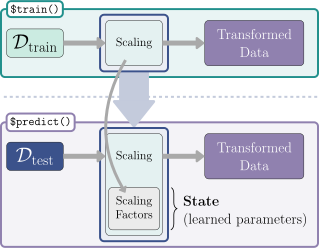
\includegraphics[width=0.7\textwidth,height=\textheight]{chapters/chapter7/Figures/mlr3book_figures-23.png}

}

\caption{\label{fig-pipelines-state}The \texttt{\$train()} method of the
``Scaling'' PipeOp both transforms data (rectangles) as well as creates
a state, which is the scaling factors necessary to transform data during
prediction.}

\end{figure}

We refer to pipelines as either sequential or non-sequential. These
terms should not be confused with ``sequential'' and ``parallel''
processing. In the context of pipelines, ``sequential'' refers to the
movement of data through the pipeline from one \texttt{PipeOp} directly
to the next from start to finish. Sequential pipelines can be visualized
in a straight line -- as we will see in this chapter. In contrast,
non-sequential pipelines see data being processed through
\texttt{PipeOp}s that may have multiple inputs and/or outputs.
Non-sequential pipelines are characterized by multiple branches so data
may be processed by different \texttt{PipeOp}s at different times.
Visually, non-sequential pipelines will not be a straight line from
start to finish, but a more complex graph. In this chapter, we will look
at sequential pipelines and in the next we will focus on non-sequential
pipelines.

\hypertarget{sec-pipelines-pipeops}{%
\section{PipeOp: Pipeline Operators}\label{sec-pipelines-pipeops}}

The basic class of \texttt{mlr3pipelines} is the
\href{https://mlr3pipelines.mlr-org.com/reference/PipeOp.html}{\texttt{PipeOp}}\index{\texttt{PipeOp}}{\marginnote{\begin{footnotesize}\texttt{PipeOp}\end{footnotesize}}},
short for ``pipeline operator''. It represents a transformative
operation on an input (for example, a training
\href{https://mlr3.mlr-org.com/reference/Task.html}{\texttt{Task}}),
resulting in some output. Similarly to a learner, it includes a
\texttt{\$train()} and a \texttt{\$predict()} method. The training phase
typically generates a particular model of the data, which is saved as
the internal
state\index{state}{\marginnote{\begin{footnotesize}State\end{footnotesize}}}.
In the prediction phase, the \texttt{PipeOp} acts on the prediction
\texttt{Task} using information from the saved state. Therefore, just
like a learner, a PipeOp has ``parameters'' (i.e., the state) that are
trained. As well as `parameters', \texttt{PipeOp}s also have
hyperparameters\index{hyperparameters} that can be set by the user when
constructing the \texttt{PipeOp} or by accessing its
\texttt{\$param\_set}. As with other classes, \texttt{PipeOp}s can be
constructed with a sugar function,
\href{https://mlr3pipelines.mlr-org.com/reference/po.html}{\texttt{po()}}\index{\texttt{po()}}{\marginnote{\begin{footnotesize}\texttt{po()}\end{footnotesize}}},
or \texttt{pos()} for multiple \texttt{PipeOp}s, and all available
\texttt{PipeOp}s are made available in the dictionary
\href{https://mlr3pipelines.mlr-org.com/reference/mlr_pipeops.html}{\texttt{mlr\_pipeops}}\index{\texttt{mlr\_pipeops}}{\marginnote{\begin{footnotesize}\texttt{mlr\_pipeops}\end{footnotesize}}}.
An up-to-date list of \texttt{PipeOp}s contained in
\texttt{mlr3pipelines} with links to their documentation can be found at
\url{https://mlr-org.com/pipeops.html}, a small subset of these are
printed below. If you want to extend \texttt{mlr3pipelines} with a
\texttt{PipeOp} that has not been implemented, have a look at our
vignette on extending \texttt{PipeOp}s by running:
\texttt{vignette("extending",\ package\ =\ "mlr3pipelines")}.

\begin{Shaded}
\begin{Highlighting}[]
\FunctionTok{as.data.table}\NormalTok{(}\FunctionTok{po}\NormalTok{())[}\DecValTok{1}\SpecialCharTok{:}\DecValTok{6}\NormalTok{, }\DecValTok{1}\SpecialCharTok{:}\DecValTok{2}\NormalTok{]}
\end{Highlighting}
\end{Shaded}

\begin{verbatim}
              key                                      label
1:         boxcox Box-Cox Transformation of Numeric Features
2:         branch                             Path Branching
3:          chunk          Chunk Input into Multiple Outputs
4: classbalancing                            Class Balancing
5:     classifavg                   Majority Vote Prediction
6:   classweights         Class Weights for Sample Weighting
\end{verbatim}

Let us now take a look at a \texttt{PipeOp} in practice using principal
component analysis\index{principal component analysis}
(PCA)\index{PCA|see{principal component analysis}} as an example, which
is implemented in
\href{https://mlr3pipelines.mlr-org.com/reference/mlr_pipeops_pca.html}{\texttt{PipeOpPCA}}.
Below we construct the \texttt{PipeOp} using its ID \texttt{"pca"} and
inspect it.

\begin{Shaded}
\begin{Highlighting}[]
\FunctionTok{library}\NormalTok{(mlr3pipelines)}

\NormalTok{po\_pca }\OtherTok{=} \FunctionTok{po}\NormalTok{(}\StringTok{"pca"}\NormalTok{, }\AttributeTok{center =} \ConstantTok{TRUE}\NormalTok{)}
\NormalTok{po\_pca}
\end{Highlighting}
\end{Shaded}

\begin{verbatim}
PipeOp: <pca> (not trained)
values: <center=TRUE>
Input channels <name [train type, predict type]>:
  input [Task,Task]
Output channels <name [train type, predict type]>:
  output [Task,Task]
\end{verbatim}

On printing, we can see that the \texttt{PipeOp} has not been trained
and that we have changed some of the hyperparameters from their default
values. The \texttt{Input\ channels} and \texttt{Output\ channels} lines
provide information about the input and output types of this PipeOp. The
PCA \texttt{PipeOp} takes one input (named ``input'') of type
``\texttt{Task}'', both during training and prediction
(``\texttt{input\ {[}Task,Task{]}}''), and produces one called
``output'' that is also of type ``\texttt{Task}'' in both phases
(``\texttt{output\ {[}Task,Task{]}}''). This highlights a key difference
from the \texttt{Learner} class: \texttt{PipeOp}s can return results
after the training phase.

A \texttt{PipeOp} can be trained using \texttt{\$train()}, which can
have multiple inputs and outputs. Both inputs and outputs are passed as
elements in a single \texttt{list}. The \texttt{"pca"} \texttt{PipeOp}
takes as input the original task and after training returns the task
with features replaced by their principal components.

\begin{Shaded}
\begin{Highlighting}[]
\NormalTok{tsk\_small }\OtherTok{=} \FunctionTok{tsk}\NormalTok{(}\StringTok{"penguins\_simple"}\NormalTok{)}\SpecialCharTok{$}\FunctionTok{select}\NormalTok{(}\FunctionTok{c}\NormalTok{(}\StringTok{"bill\_depth"}\NormalTok{, }\StringTok{"bill\_length"}\NormalTok{))}
\NormalTok{poin }\OtherTok{=} \FunctionTok{list}\NormalTok{(tsk\_small}\SpecialCharTok{$}\FunctionTok{clone}\NormalTok{()}\SpecialCharTok{$}\FunctionTok{filter}\NormalTok{(}\DecValTok{1}\SpecialCharTok{:}\DecValTok{5}\NormalTok{))}
\NormalTok{poout }\OtherTok{=}\NormalTok{ po\_pca}\SpecialCharTok{$}\FunctionTok{train}\NormalTok{(poin) }\CommentTok{\# poin: Task in a list}
\NormalTok{poout }\CommentTok{\# list with a single element \textquotesingle{}output\textquotesingle{}}
\end{Highlighting}
\end{Shaded}

\begin{verbatim}
$output
<TaskClassif:penguins> (5 x 3): Simplified Palmer Penguins
* Target: species
* Properties: multiclass
* Features (2):
  - dbl (2): PC1, PC2
\end{verbatim}

\begin{Shaded}
\begin{Highlighting}[]
\NormalTok{poout[[}\DecValTok{1}\NormalTok{]]}\SpecialCharTok{$}\FunctionTok{head}\NormalTok{()}
\end{Highlighting}
\end{Shaded}

\begin{verbatim}
   species     PC1       PC2
1:  Adelie  0.1561  0.005716
2:  Adelie  1.2677  0.789534
3:  Adelie  1.5336 -0.174460
4:  Adelie -2.1096  0.998977
5:  Adelie -0.8478 -1.619768
\end{verbatim}

During training, PCA transforms incoming data by rotating it in such a
way that features become uncorrelated and are ordered by their
contribution to the total variance. The rotation matrix is also saved in
the internal \texttt{\$state} field during training (shown in
Figure~\ref{fig-pipelines-state}), which is then used during predictions
and applied to new data.

\begin{Shaded}
\begin{Highlighting}[]
\NormalTok{po\_pca}\SpecialCharTok{$}\NormalTok{state}
\end{Highlighting}
\end{Shaded}

\begin{verbatim}
Standard deviations (1, .., p=2):
[1] 1.513 1.034

Rotation (n x k) = (2 x 2):
                PC1     PC2
bill_depth  -0.6116 -0.7911
bill_length  0.7911 -0.6116
\end{verbatim}

Once trained, the \texttt{\$predict()} function can then access the
saved state to operate on the test data, which again is passed as a
\texttt{list}:

\begin{Shaded}
\begin{Highlighting}[]
\NormalTok{tsk\_onepenguin }\OtherTok{=}\NormalTok{ tsk\_small}\SpecialCharTok{$}\FunctionTok{clone}\NormalTok{()}\SpecialCharTok{$}\FunctionTok{filter}\NormalTok{(}\DecValTok{42}\NormalTok{)}
\NormalTok{poin }\OtherTok{=} \FunctionTok{list}\NormalTok{(tsk\_onepenguin)}
\NormalTok{poout }\OtherTok{=}\NormalTok{ po\_pca}\SpecialCharTok{$}\FunctionTok{predict}\NormalTok{(poin)}
\NormalTok{poout[[}\DecValTok{1}\NormalTok{]]}\SpecialCharTok{$}\FunctionTok{data}\NormalTok{()}
\end{Highlighting}
\end{Shaded}

\begin{verbatim}
   species   PC1    PC2
1:  Adelie 1.555 -1.455
\end{verbatim}

\hypertarget{sec-pipelines-graphs}{%
\section{Graph: Networks of PipeOps}\label{sec-pipelines-graphs}}

\texttt{PipeOp}s represent individual computational steps in machine
learning pipelines. These pipelines themselves are defined by
\href{https://mlr3pipelines.mlr-org.com/reference/Graph.html}{\texttt{Graph}}\index{\texttt{Graph}}
objects. A \texttt{Graph} is a collection of \texttt{PipeOp}s with
``edges'' that guide the flow of data.

The most convenient way of building a \texttt{Graph} is to connect a
sequence of \texttt{PipeOp}s using the
\texttt{\%\textgreater{}\textgreater{}\%}-operator
{\marginnote{\begin{footnotesize}\texttt{\%\textgreater{}\textgreater{}\%}\end{footnotesize}}}
\index{\%>>\%} (read ``double-arrow'') operator. When given two
\texttt{PipeOp}s, this operator creates a \texttt{Graph} that first
executes the left-hand \texttt{PipeOp}, followed by the right-hand one.
It can also be used to connect a \texttt{Graph} with a \texttt{PipeOp},
or with another \texttt{Graph}. The following example uses
\texttt{po("mutate")} to add a new feature to the task, and
\texttt{po("scale")} to then scale\index{scale} and center all numeric
features.

\begin{Shaded}
\begin{Highlighting}[]
\NormalTok{po\_mutate }\OtherTok{=} \FunctionTok{po}\NormalTok{(}\StringTok{"mutate"}\NormalTok{,}
  \AttributeTok{mutation =} \FunctionTok{list}\NormalTok{(}\AttributeTok{bill\_ratio =} \SpecialCharTok{\textasciitilde{}}\NormalTok{bill\_length }\SpecialCharTok{/}\NormalTok{ bill\_depth)}
\NormalTok{)}
\NormalTok{po\_scale }\OtherTok{=} \FunctionTok{po}\NormalTok{(}\StringTok{"scale"}\NormalTok{)}
\NormalTok{graph }\OtherTok{=}\NormalTok{ po\_mutate }\SpecialCharTok{\%\textgreater{}\textgreater{}\%}\NormalTok{ po\_scale}
\NormalTok{graph}
\end{Highlighting}
\end{Shaded}

\begin{verbatim}
Graph with 2 PipeOps:
     ID         State sccssors prdcssors
 mutate <<UNTRAINED>>    scale          
  scale <<UNTRAINED>>             mutate
\end{verbatim}

The output provides information about the layout of the Graph. For each
\texttt{PipOp} (\texttt{ID}), we can see information about the state
(\texttt{State}), as well as a list of its successors
(\texttt{sccssors}), which are \texttt{PipeOp}s that come directly after
the given \texttt{PipeOp}, and its predecessors (\texttt{prdcssors}),
the \texttt{PipeOp}s that are connected to its input. In this simple
\texttt{Graph}, the output of the \texttt{"mutate"} \texttt{PipeOp} is
passed directly to the \texttt{"scale"} \texttt{PipeOp} and neither
takes any other inputs or outputs from other \texttt{PipeOp}s. The
\texttt{\$plot()}\index{\texttt{Graph}!\texttt{\$plot()}}{\marginnote{\begin{footnotesize}\$plot()\end{footnotesize}}}
method can be used to visualize the graph.

\begin{Shaded}
\begin{Highlighting}[]
\NormalTok{graph}\SpecialCharTok{$}\FunctionTok{plot}\NormalTok{(}\AttributeTok{horizontal =} \ConstantTok{TRUE}\NormalTok{)}
\end{Highlighting}
\end{Shaded}

\begin{figure}

{\centering \includegraphics[width=1\textwidth,height=\textheight]{chapters/chapter7/sequential_pipelines_files/figure-pdf/fig-pipelines-basic-plot-1.png}

}

\caption{\label{fig-pipelines-basic-plot}Simple sequential pipeline
plot.}

\end{figure}

The plot demonstrates how a \texttt{Graph} is simply a collection of
\texttt{PipeOp}s that are connected by `edges'. The collection of
\texttt{PipeOp}s inside a \texttt{Graph} can be accessed through the
\texttt{\$pipeops} \index{\$pipeops} field. The \texttt{\$edges}
\index{\$edges} field can be used to access edges, which returns a
\texttt{data.table} listing the ``source'' (\texttt{src\_id},
\texttt{src\_channel}) and ``destination'' (\texttt{dst\_id},
\texttt{dst\_channel}) of data flowing along each edge
{\marginnote{\begin{footnotesize}\texttt{\$edges}/\texttt{\$pipeops}\end{footnotesize}}}.

\begin{Shaded}
\begin{Highlighting}[]
\NormalTok{graph}\SpecialCharTok{$}\NormalTok{pipeops}
\end{Highlighting}
\end{Shaded}

\begin{verbatim}
$mutate
PipeOp: <mutate> (not trained)
values: <mutation=<list>, delete_originals=FALSE>
Input channels <name [train type, predict type]>:
  input [Task,Task]
Output channels <name [train type, predict type]>:
  output [Task,Task]

$scale
PipeOp: <scale> (not trained)
values: <robust=FALSE>
Input channels <name [train type, predict type]>:
  input [Task,Task]
Output channels <name [train type, predict type]>:
  output [Task,Task]
\end{verbatim}

\begin{Shaded}
\begin{Highlighting}[]
\NormalTok{graph}\SpecialCharTok{$}\NormalTok{edges}
\end{Highlighting}
\end{Shaded}

\begin{verbatim}
   src_id src_channel dst_id dst_channel
1: mutate      output  scale       input
\end{verbatim}

Instead of using \texttt{\%\textgreater{}\textgreater{}\%}, you can also
create a \texttt{Graph} explicitly using the \texttt{\$add\_pipeop()}
and \texttt{\$add\_edge()} methods to create \texttt{PipeOp}s and the
edges connecting them:

\begin{Shaded}
\begin{Highlighting}[]
\NormalTok{graph }\OtherTok{=}\NormalTok{ Graph}\SpecialCharTok{$}\FunctionTok{new}\NormalTok{()}\SpecialCharTok{$}
  \FunctionTok{add\_pipeop}\NormalTok{(po\_mutate)}\SpecialCharTok{$}
  \FunctionTok{add\_pipeop}\NormalTok{(po\_scale)}\SpecialCharTok{$}
  \FunctionTok{add\_edge}\NormalTok{(}\StringTok{"mutate"}\NormalTok{, }\StringTok{"scale"}\NormalTok{)}
\end{Highlighting}
\end{Shaded}

\begin{tcolorbox}[enhanced jigsaw, opacitybacktitle=0.6, rightrule=.15mm, opacityback=0, arc=.35mm, breakable, titlerule=0mm, colframe=quarto-callout-tip-color-frame, coltitle=black, bottomrule=.15mm, toprule=.15mm, colback=white, colbacktitle=quarto-callout-tip-color!10!white, bottomtitle=1mm, toptitle=1mm, title=\textcolor{quarto-callout-tip-color}{\faLightbulb}\hspace{0.5em}{Graphs and DAGs}, leftrule=.75mm, left=2mm]

The
\href{https://mlr3pipelines.mlr-org.com/reference/Graph.html}{\texttt{Graph}}
class represents an object similar to a directed acyclic
graph\index{directed acyclic graph}
(DAG)\index{DAG|see{Directed Acyclic Graph}}, since the input of a
\href{https://mlr3pipelines.mlr-org.com/reference/PipeOp.html}{\texttt{PipeOp}}
cannot depend on its output and hence cycles are not allowed. However,
the resemblance to a DAG is not perfect, since the \texttt{Graph} class
allows for multiple edges between nodes. A term such as ``directed
acyclic multigraph'' would be more accurate, but we use ``graph'' for
simplicity.

\end{tcolorbox}

Once built, a \texttt{Graph} can be used by calling \texttt{\$train()}
and \texttt{\$predict()} as if it were a \texttt{Learner} (though it
still outputs a \texttt{list} during training and prediction):

\begin{Shaded}
\begin{Highlighting}[]
\NormalTok{result }\OtherTok{=}\NormalTok{ graph}\SpecialCharTok{$}\FunctionTok{train}\NormalTok{(tsk\_small)}
\NormalTok{result}
\end{Highlighting}
\end{Shaded}

\begin{verbatim}
$scale.output
<TaskClassif:penguins> (333 x 4): Simplified Palmer Penguins
* Target: species
* Properties: multiclass
* Features (3):
  - dbl (3): bill_depth, bill_length, bill_ratio
\end{verbatim}

\begin{Shaded}
\begin{Highlighting}[]
\NormalTok{result[[}\DecValTok{1}\NormalTok{]]}\SpecialCharTok{$}\FunctionTok{data}\NormalTok{()[}\DecValTok{1}\SpecialCharTok{:}\DecValTok{3}\NormalTok{]}
\end{Highlighting}
\end{Shaded}

\begin{verbatim}
   species bill_depth bill_length bill_ratio
1:  Adelie     0.7796     -0.8947    -1.0421
2:  Adelie     0.1194     -0.8216    -0.6804
3:  Adelie     0.4241     -0.6753    -0.7435
\end{verbatim}

\begin{Shaded}
\begin{Highlighting}[]
\NormalTok{result }\OtherTok{=}\NormalTok{ graph}\SpecialCharTok{$}\FunctionTok{predict}\NormalTok{(tsk\_onepenguin)}
\NormalTok{result[[}\DecValTok{1}\NormalTok{]]}\SpecialCharTok{$}\FunctionTok{head}\NormalTok{()}
\end{Highlighting}
\end{Shaded}

\begin{verbatim}
   species bill_depth bill_length bill_ratio
1:  Adelie     0.9319      -0.529    -0.8963
\end{verbatim}

\hypertarget{sec-pipelines-sequential}{%
\section{Sequential Learner-Pipelines}\label{sec-pipelines-sequential}}

Possibly the most common application for \texttt{mlr3pipelines} is to
use it to perform preprocessing\index{preprocessing} tasks, such as
missing value imputation\index{imputation} or factor
encoding\index{factor encoding}, and to then feed the resulting data
into a \texttt{Learner} -- we will see more of this in practice in
Chapter~\ref{sec-preprocessing}. A \texttt{Graph} representing this
workflow manipulates data and fits a \texttt{Learner}-model during
training, ensuring that the data is processed the same way during the
prediction stage. Conceptually, the process may look as shown in
Figure~\ref{fig-pipelines-pipeline}.

\begin{figure}

{\centering 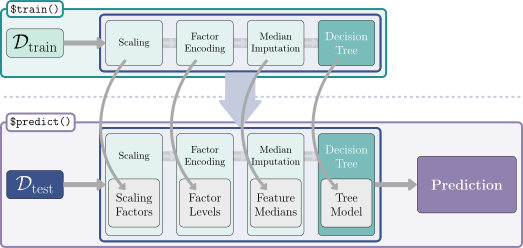
\includegraphics[width=1\textwidth,height=\textheight]{chapters/chapter7/Figures/mlr3book_figures-22.png}

}

\caption{\label{fig-pipelines-pipeline}Conceptualization of training and
prediction process inside a sequential learner-pipeline. During training
(top row), the data is passed along the preprocessing operators, each of
which modifies the data and creates a \texttt{\$state}. Finally, the
learner receives the data and a model is created. During prediction
(bottom row), data is likewise transformed by preprocessing operators,
using their respective \texttt{\$state} (gray boxes) information in the
process. The learner then receives data that has the same format as the
data seen during training, and makes a prediction.}

\end{figure}

\hypertarget{learners-as-pipeops-and-graphs-as-learners}{%
\subsection{Learners as PipeOps and Graphs as
Learners}\label{learners-as-pipeops-and-graphs-as-learners}}

In Figure~\ref{fig-pipelines-pipeline} the final \texttt{PipeOp} is a
\texttt{Learner}. \texttt{Learner} objects can be converted to
\texttt{PipeOp}s with
\href{https://mlr3pipelines.mlr-org.com/reference/as_pipeop.html}{\texttt{as\_pipeop()}},
however, this is only necessary if you choose to manually create a graph
instead of using \texttt{\%\textgreater{}\textgreater{}\%}. With either
method, internally \texttt{Learner}s are passed to
\texttt{po("learner")}. The following code creates a
\href{https://mlr3pipelines.mlr-org.com/reference/Graph.html}{\texttt{Graph}}
that uses \texttt{po("imputesample")} to impute\index{imputation}
missing values by sampling from observed values
(Section~\ref{sec-preprocessing-missing}) then fits a logistic
regression\index{logistic regression} on the transformed task.

\begin{Shaded}
\begin{Highlighting}[]
\NormalTok{lrn\_logreg }\OtherTok{=} \FunctionTok{lrn}\NormalTok{(}\StringTok{"classif.log\_reg"}\NormalTok{)}
\NormalTok{graph }\OtherTok{=} \FunctionTok{po}\NormalTok{(}\StringTok{"imputesample"}\NormalTok{) }\SpecialCharTok{\%\textgreater{}\textgreater{}\%}\NormalTok{ lrn\_logreg}
\NormalTok{graph}\SpecialCharTok{$}\FunctionTok{plot}\NormalTok{(}\AttributeTok{horizontal =} \ConstantTok{TRUE}\NormalTok{)}
\end{Highlighting}
\end{Shaded}

\begin{figure}

{\centering \includegraphics[width=1\textwidth,height=\textheight]{chapters/chapter7/sequential_pipelines_files/figure-pdf/fig-pipelines-learnerpipeop-1.png}

}

\caption{\label{fig-pipelines-learnerpipeop}\texttt{"imputesample"} and
\texttt{"learner"} PipeOps in a sequential pipeline.}

\end{figure}

We have seen how training and predicting \texttt{Graph}s is possible but
has a slightly different design to \texttt{Learner} objects, i.e.,
inputs and outputs during both training and predicting are \texttt{list}
objects. To use a \texttt{Graph} as a \texttt{Learner} with an identical
interface, it can be wrapped in a
\href{https://mlr3pipelines.mlr-org.com/reference/mlr_learners_graph.html}{\texttt{GraphLearner}}\index{\texttt{GraphLearner}}
object with
\href{https://mlr3.mlr-org.com/reference/as_learner.html}{\texttt{as\_learner()}}\index{\texttt{as\_learner()}}{\marginnote{\begin{footnotesize}\texttt{GraphLearner}\end{footnotesize}}}.
The \texttt{Graph} can then be used like any other \texttt{Learner}, so
now we can benchmark our pipeline to decide if we should impute by
sampling or with the mode of observed values
(\texttt{po("imputemode")}):

\begin{Shaded}
\begin{Highlighting}[]
\NormalTok{glrn\_sample }\OtherTok{=} \FunctionTok{as\_learner}\NormalTok{(graph)}
\NormalTok{glrn\_mode }\OtherTok{=} \FunctionTok{as\_learner}\NormalTok{(}\FunctionTok{po}\NormalTok{(}\StringTok{"imputemode"}\NormalTok{) }\SpecialCharTok{\%\textgreater{}\textgreater{}\%}\NormalTok{ lrn\_logreg)}

\NormalTok{design }\OtherTok{=} \FunctionTok{benchmark\_grid}\NormalTok{(}\FunctionTok{tsk}\NormalTok{(}\StringTok{"pima"}\NormalTok{), }\FunctionTok{list}\NormalTok{(glrn\_sample, glrn\_mode),}
  \FunctionTok{rsmp}\NormalTok{(}\StringTok{"cv"}\NormalTok{, }\AttributeTok{folds =} \DecValTok{3}\NormalTok{))}
\NormalTok{bmr }\OtherTok{=} \FunctionTok{benchmark}\NormalTok{(design)}
\NormalTok{aggr }\OtherTok{=}\NormalTok{ bmr}\SpecialCharTok{$}\FunctionTok{aggregate}\NormalTok{()[, .(learner\_id, classif.ce)]}
\NormalTok{aggr}
\end{Highlighting}
\end{Shaded}

\begin{verbatim}
                     learner_id classif.ce
1: imputesample.classif.log_reg     0.2357
2:   imputemode.classif.log_reg     0.2396
\end{verbatim}

In this example, we can see that the sampling imputation method worked
slightly better, although the difference is likely not significant.

\begin{tcolorbox}[enhanced jigsaw, opacitybacktitle=0.6, rightrule=.15mm, opacityback=0, arc=.35mm, breakable, titlerule=0mm, colframe=quarto-callout-tip-color-frame, coltitle=black, bottomrule=.15mm, toprule=.15mm, colback=white, colbacktitle=quarto-callout-tip-color!10!white, bottomtitle=1mm, toptitle=1mm, title=\textcolor{quarto-callout-tip-color}{\faLightbulb}\hspace{0.5em}{Automatic Conversion to Learner}, leftrule=.75mm, left=2mm]

In this book, we always use \texttt{as\_learner()} to convert a
\texttt{Graph} to a \texttt{Learner} explicitly for clarity. While this
conversion is necessary when you want to use \texttt{Learner}-specific
functions like \texttt{\$predict\_newdata()}, builtin \texttt{mlr3}
methods like \texttt{resample()} and \texttt{benchmark\_grid()} will
make this conversion automatically and it is therefore not strictly
needed. In the above example, it is therefore also possible to use

\begin{Shaded}
\begin{Highlighting}[]
\NormalTok{design }\OtherTok{=} \FunctionTok{benchmark\_grid}\NormalTok{(}\FunctionTok{tsk}\NormalTok{(}\StringTok{"pima"}\NormalTok{),}
  \FunctionTok{list}\NormalTok{(graph, }\FunctionTok{po}\NormalTok{(}\StringTok{"imputesample"}\NormalTok{) }\SpecialCharTok{\%\textgreater{}\textgreater{}\%}\NormalTok{ lrn\_logreg),}
  \FunctionTok{rsmp}\NormalTok{(}\StringTok{"cv"}\NormalTok{, }\AttributeTok{folds =} \DecValTok{3}\NormalTok{))}
\end{Highlighting}
\end{Shaded}

\end{tcolorbox}

\hypertarget{inspecting-graphs}{%
\subsection{Inspecting Graphs}\label{inspecting-graphs}}

You may want to inspect pipelines and the flow of data to learn more
about your pipeline or to debug\index{debugging} them. We first need to
set the \texttt{\$keep\_results} flag to be \texttt{TRUE} so that
intermediate results are retained, which is turned off by default to
save memory.

\begin{Shaded}
\begin{Highlighting}[]
\NormalTok{glrn\_sample}\SpecialCharTok{$}\NormalTok{graph\_model}\SpecialCharTok{$}\NormalTok{keep\_results }\OtherTok{=} \ConstantTok{TRUE}
\NormalTok{glrn\_sample}\SpecialCharTok{$}\FunctionTok{train}\NormalTok{(}\FunctionTok{tsk}\NormalTok{(}\StringTok{"pima"}\NormalTok{))}
\end{Highlighting}
\end{Shaded}

The \texttt{Graph} can be accessed through the \texttt{\$graph\_model}
field and then \texttt{PipeOp}s can be accessed with \texttt{\$pipeops}
as before. In this example, we can see that our
\href{https://mlr3.mlr-org.com/reference/Task.html}{\texttt{Task}} no
longer has missing data after training the \texttt{"imputesample"}
\texttt{PipeOp}. This can be used to access arbitrary intermediate
results:

\begin{Shaded}
\begin{Highlighting}[]
\NormalTok{imputesample\_output }\OtherTok{=}\NormalTok{ glrn\_sample}\SpecialCharTok{$}\NormalTok{graph\_model}\SpecialCharTok{$}\NormalTok{pipeops}\SpecialCharTok{$}\NormalTok{imputesample}\SpecialCharTok{$}
\NormalTok{  .result}
\NormalTok{imputesample\_output[[}\DecValTok{1}\NormalTok{]]}\SpecialCharTok{$}\FunctionTok{missings}\NormalTok{()}
\end{Highlighting}
\end{Shaded}

\begin{verbatim}
diabetes      age pedigree pregnant  glucose  insulin     mass pressure 
       0        0        0        0        0        0        0        0 
 triceps 
       0 
\end{verbatim}

We could also use \texttt{\$pipeops} to access our underlying
\href{https://mlr3.mlr-org.com/reference/Learner.html}{\texttt{Learner}},
note we need to use \texttt{\$learner\_model} to get the learner from
the
\href{https://mlr3pipelines.mlr-org.com/reference/mlr_pipeops_learner.html}{\texttt{PipeOpLearner}}.
We could use a similar method to peek at the state of any
\texttt{PipeOp} in the graph:

\begin{Shaded}
\begin{Highlighting}[]
\NormalTok{pipeop\_logreg }\OtherTok{=}\NormalTok{ glrn\_sample}\SpecialCharTok{$}\NormalTok{graph\_model}\SpecialCharTok{$}\NormalTok{pipeops}\SpecialCharTok{$}\NormalTok{classif.log\_reg}
\NormalTok{learner\_logreg }\OtherTok{=}\NormalTok{ pipeop\_logreg}\SpecialCharTok{$}\NormalTok{learner\_model}
\NormalTok{learner\_logreg}
\end{Highlighting}
\end{Shaded}

\begin{verbatim}
<LearnerClassifLogReg:classif.log_reg>
* Model: glm
* Parameters: list()
* Packages: mlr3, mlr3learners, stats
* Predict Types:  [response], prob
* Feature Types: logical, integer, numeric, character, factor,
  ordered
* Properties: loglik, twoclass
\end{verbatim}

\begin{tcolorbox}[enhanced jigsaw, opacitybacktitle=0.6, rightrule=.15mm, opacityback=0, arc=.35mm, breakable, titlerule=0mm, colframe=quarto-callout-tip-color-frame, coltitle=black, bottomrule=.15mm, toprule=.15mm, colback=white, colbacktitle=quarto-callout-tip-color!10!white, bottomtitle=1mm, toptitle=1mm, title=\textcolor{quarto-callout-tip-color}{\faLightbulb}\hspace{0.5em}{\texttt{\$base\_learner()}}, leftrule=.75mm, left=2mm]

In this example we could have used
\texttt{glrn\_sample\$base\_learner()} to immediately access our trained
learner, however, this does not generalize to more complex pipelines
that may contain multiple learners.

\end{tcolorbox}

\hypertarget{configuring-pipeline-hyperparameters}{%
\subsection{Configuring Pipeline
Hyperparameters}\label{configuring-pipeline-hyperparameters}}

\texttt{PipeOp} hyperparameters are collected together in the
\texttt{\$param\_set} of a graph and prefixed with the ID of the
\texttt{PipeOp} to avoid parameter name clashes. Below we use the same
\texttt{PipeOp} twice but set the \texttt{id} to ensure their IDs are
unique.

\begin{Shaded}
\begin{Highlighting}[]
\NormalTok{graph }\OtherTok{=} \FunctionTok{po}\NormalTok{(}\StringTok{"scale"}\NormalTok{, }\AttributeTok{center =} \ConstantTok{FALSE}\NormalTok{, }\AttributeTok{scale =} \ConstantTok{TRUE}\NormalTok{, }\AttributeTok{id =} \StringTok{"scale"}\NormalTok{) }\SpecialCharTok{\%\textgreater{}\textgreater{}\%}
  \FunctionTok{po}\NormalTok{(}\StringTok{"scale"}\NormalTok{, }\AttributeTok{center =} \ConstantTok{TRUE}\NormalTok{, }\AttributeTok{scale =} \ConstantTok{FALSE}\NormalTok{, }\AttributeTok{id =} \StringTok{"center"}\NormalTok{) }\SpecialCharTok{\%\textgreater{}\textgreater{}\%}
  \FunctionTok{lrn}\NormalTok{(}\StringTok{"classif.rpart"}\NormalTok{, }\AttributeTok{cp =} \DecValTok{1}\NormalTok{)}
\FunctionTok{unlist}\NormalTok{(graph}\SpecialCharTok{$}\NormalTok{param\_set}\SpecialCharTok{$}\NormalTok{values)}
\end{Highlighting}
\end{Shaded}

\begin{verbatim}
      scale.robust       scale.center        scale.scale 
                 0                  0                  1 
     center.robust      center.center       center.scale 
                 0                  1                  0 
classif.rpart.xval   classif.rpart.cp 
                 0                  1 
\end{verbatim}

\begin{tcolorbox}[enhanced jigsaw, opacitybacktitle=0.6, rightrule=.15mm, opacityback=0, arc=.35mm, breakable, titlerule=0mm, colframe=quarto-callout-warning-color-frame, coltitle=black, bottomrule=.15mm, toprule=.15mm, colback=white, colbacktitle=quarto-callout-warning-color!10!white, bottomtitle=1mm, toptitle=1mm, title=\textcolor{quarto-callout-warning-color}{\faExclamationTriangle}\hspace{0.5em}{PipeOp IDs in Graphs}, leftrule=.75mm, left=2mm]

If you need to change the ID of a
\href{https://mlr3pipelines.mlr-org.com/reference/PipeOp.html}{\texttt{PipeOp}}
in a
\href{https://mlr3pipelines.mlr-org.com/reference/Graph.html}{\texttt{Graph}}
then use the \texttt{\$set\_names} method from the \texttt{Graph} class,
e.g.,
\texttt{some\_graph\$set\_names(old\ =\ "old\_name",\ new\ =\ "new\_name")}.
Do not change the ID of a \texttt{PipeOp} through
\texttt{graph\$pipeops\$\textless{}old\_id\textgreater{}\$id\ =\ \textless{}new\_id\textgreater{}},
as this will only alter the \texttt{PipeOp}'s record of its own ID, and
not the \texttt{Graph}'s record, which will lead to errors.

\end{tcolorbox}

Whether a pipeline is treated as a \texttt{Graph} or
\texttt{GraphLearner}, hyperparameters\index{hyperparameters} are
updated and accessed in the same way.

\begin{Shaded}
\begin{Highlighting}[]
\NormalTok{graph}\SpecialCharTok{$}\NormalTok{param\_set}\SpecialCharTok{$}\NormalTok{values}\SpecialCharTok{$}\NormalTok{classif.rpart.maxdepth }\OtherTok{=} \DecValTok{5}
\NormalTok{graph\_learner }\OtherTok{=} \FunctionTok{as\_learner}\NormalTok{(graph)}
\NormalTok{graph\_learner}\SpecialCharTok{$}\NormalTok{param\_set}\SpecialCharTok{$}\NormalTok{values}\SpecialCharTok{$}\NormalTok{classif.rpart.minsplit }\OtherTok{=} \DecValTok{2}
\FunctionTok{unlist}\NormalTok{(graph\_learner}\SpecialCharTok{$}\NormalTok{param\_set}\SpecialCharTok{$}\NormalTok{values)}
\end{Highlighting}
\end{Shaded}

\begin{verbatim}
          scale.center            scale.scale           scale.robust 
                     0                      1                      0 
         center.center           center.scale          center.robust 
                     1                      0                      0 
      classif.rpart.cp classif.rpart.maxdepth classif.rpart.minsplit 
                     1                      5                      2 
    classif.rpart.xval 
                     0 
\end{verbatim}

\hypertarget{conclusion-5}{%
\section{Conclusion}\label{conclusion-5}}

In this chapter, we introduced
\href{https://mlr3pipelines.mlr-org.com}{\texttt{mlr3pipelines}}\index{\texttt{mlr3pipelines}}
and its building blocks:
\href{https://mlr3pipelines.mlr-org.com/reference/Graph.html}{\texttt{Graph}}
and
\href{https://mlr3pipelines.mlr-org.com/reference/PipeOp.html}{\texttt{PipeOp}}.
We saw how to create pipelines as \texttt{Graph} objects from multiple
\texttt{PipeOp} objects and how to access \texttt{PipeOp}s from a
\texttt{Graph}. We also saw how to treat a \texttt{Learner} as a
\texttt{PipeOp} and how to treat a \texttt{Graph} as a \texttt{Learner}.
In Chapter~\ref{sec-pipelines-nonseq} we will take this functionality a
step further and look at pipelines where \texttt{PipeOp}s are not
executed sequentially, as well as looking at how you can use
\href{https://mlr3tuning.mlr-org.com}{\texttt{mlr3tuning}}\index{\texttt{mlr3tuning}}
to tune pipelines. A lot of practical examples that use sequential
pipelines can be found in Chapter~\ref{sec-preprocessing} where we look
at pipelines for data preprocessing.

\hypertarget{tbl-api-pipelines-seq}{}
\begin{longtable}[]{@{}
  >{\raggedright\arraybackslash}p{(\columnwidth - 4\tabcolsep) * \real{0.3333}}
  >{\raggedright\arraybackslash}p{(\columnwidth - 4\tabcolsep) * \real{0.3333}}
  >{\raggedright\arraybackslash}p{(\columnwidth - 4\tabcolsep) * \real{0.3333}}@{}}
\caption{\label{tbl-api-pipelines-seq}Important classes and functions
covered in this chapter with underlying class (if applicable), class
constructor or function, and important class fields and methods (if
applicable).}\tabularnewline
\toprule\noalign{}
\begin{minipage}[b]{\linewidth}\raggedright
Class
\end{minipage} & \begin{minipage}[b]{\linewidth}\raggedright
Constructor/Function
\end{minipage} & \begin{minipage}[b]{\linewidth}\raggedright
Fields/Methods
\end{minipage} \\
\midrule\noalign{}
\endfirsthead
\toprule\noalign{}
\begin{minipage}[b]{\linewidth}\raggedright
Class
\end{minipage} & \begin{minipage}[b]{\linewidth}\raggedright
Constructor/Function
\end{minipage} & \begin{minipage}[b]{\linewidth}\raggedright
Fields/Methods
\end{minipage} \\
\midrule\noalign{}
\endhead
\bottomrule\noalign{}
\endlastfoot
\href{https://mlr3pipelines.mlr-org.com/reference/PipeOp.html}{\texttt{PipeOp}}
&
\href{https://mlr3pipelines.mlr-org.com/reference/po.html}{\texttt{po()}}
& \texttt{\$train()}; \texttt{\$predict()}; \texttt{\$state};
\texttt{\$id}; \texttt{\$param\_set} \\
\href{https://mlr3pipelines.mlr-org.com/reference/Graph.html}{\texttt{Graph}}
& \texttt{\%\textgreater{}\textgreater{}\%} & \texttt{\$add\_pipeop()};
\texttt{\$add\_edge()}; \texttt{\$pipeops};
\texttt{\$edges};\texttt{\$train()}; \texttt{\$predict()} \\
\href{https://mlr3pipelines.mlr-org.com/reference/mlr_learners_graph.html}{\texttt{GraphLearner}}
&
\href{https://mlr3.mlr-org.com/reference/as_learner.html}{\texttt{as\_learner}}
& \texttt{\$graph} \\
\href{https://mlr3pipelines.mlr-org.com/reference/mlr_pipeops_learner.html}{\texttt{PipeOpLearner}}
&
\href{https://mlr3pipelines.mlr-org.com/reference/as_pipeop.html}{\texttt{as\_pipeop}}
& \texttt{\$learner\_model} \\
\end{longtable}

\hypertarget{exercises-5}{%
\section{Exercises}\label{exercises-5}}

\begin{enumerate}
\def\labelenumi{\arabic{enumi}.}
\tightlist
\item
  Create a learner containing a \texttt{Graph} that first imputes
  missing values using \texttt{po("imputeoor")}, standardizes the data
  using \texttt{po("scale")}, and then fits a logistic linear model
  using \texttt{"lrn("classif.log\_reg")}.
\item
  Train the learner created in the previous exercise on
  \texttt{tsk("pima")} and display the coefficients of the resulting
  model. What are two different ways to access the model?
\item
  Verify that the \texttt{"age"} column of the input task of
  \texttt{"lrn("classif.log\_reg")} from the previous exercise is indeed
  standardized. One way to do this would be to look at the
  \texttt{\$data} field of the \texttt{lrn("classif.log\_reg")} model;
  however, that is specific to that particular learner and does not work
  in general. What would be a different, more general way to do this?
  Hint: use the \texttt{\$keep\_results} flag.
\end{enumerate}
